%Chapter 7

\chapter{On the Transferability of Deep-Q Networks} % Chapter title
\label{ch:dqn_transfer} % For referencing the chapter elsewhere, use \autoref{ch:introduction} 

\begin{remark}{Outline}
\end{remark}




\section{Motivation}


\section{A large-scale Empirical Study}
\label{sec:empirical_study}

# Mention similarities and dissimilarities among games

\subsection{Experimental Setup}

\subsection{Results}

When analyzing the performance of fine-tuned models, more exciting results have been obtained. Specifically, we have noticed that this approach can result in one out of three possible TL types. We classify them as follows:

\begin{itemize}
	\item\textcolor{RoyalBlue}{Negative-TL}: this is a training scenario in which it is counterproductive to start solving the problem modeled by $\mathcal{M}_t$ with a network that is pre-trained on $\mathcal{M}_s$. The most beneficial strategy instead is to train a randomly initialized network from scratch. We can visually observe how this type of TL presents itself in the first plot of Fig. \ref{fig:types_of_tl}, where we report the TL performance of a model which is pre-trained on \texttt{BankHeist} and is fine-tuned on \texttt{FishingDerby}.
   We can observe that over $\approx 3000$ training episodes, the cumulative reward obtained by the \texttt{BankHeist} model is significantly lower than the one obtained by a randomly initialized model.        
    
    \item\textcolor{RoyalBlue}{Absent-TL}: this training scenario does not present significant benefits, nor particular drawbacks when a pre-trained network is trained on $\mathcal{M}_t$ instead of a randomly initialized one. We report an example of this TL scenario in the central plot of Fig. \ref{fig:types_of_tl} where a \texttt{BankHeist} model gets fine-tuned on the \texttt{Boxing} game. We can easily observe that there are no significant differences between the performance of the two networks. While the final network's performance is not as bad as the one obtained when the previous TL scenario occurs, Absent-TL is still not desirable since there are no practical benefits that can motivate the effort required for pre-training a Deep Q-Network on a source-task.
    
    \item\textcolor{RoyalBlue}{Positive-TL}: this corresponds to the most desirable outcome that can be achieved when a pre-trained network gets fine-tuned on the target-task. As reviewed in Chapter \ref{ch:transfer_learning} TL has three main objectives: `Learning speed Improvements", `Asymptotic Improvements" and `Jumpstart Improvements". We show how the first two of these improvements can appear in DRL in the last plot of Fig. \ref{fig:types_of_tl}, where a model pre-trained on \texttt{BankHeist} can significantly outperform a model that is trained from scratch on the \texttt{Enduro} environment. We can observe a \textit{Learning speed Improvement} since the \texttt{BankHeist} model starts improving its policy already after $\approx 50$ epochs, while at the same time, there also is \textit{Asymptotic Improvement} since the cumulative reward that is obtained by the networks is significantly higher than the one that is obtained by an agent trained from scratch. 
\end{itemize}



\section{Control Experiments}

The results presented in the previous section seem to be questioning the level of transferability of convolutional neural networks that get trained for solving RL tasks. In fact, the training strategy of fine-tuning a pre-trained model on $\mathcal{M}_T$ does not result in the same type of performance gains that we have extensively observed throughout the first part of this dissertation, when pre-trained models were transferred and fine-tuned in a supervised learning context. To better characterize the transfer learning properties of pre-trained convolutional neural networks for DRL, we have designed a set of simple control experiments that allow us to examine their transfer learning behavior in training conditions that are as similar as possible to the ones that have characterized the experimental setup adopted in Sec. \ref{sec:empirical_study}. The main difference, however, is that the RL tasks that will be considered from now on, are much simpler than the ones defined within the ALE environment, and therefore do not require extraordinarily long training times for learning an optimal policy.   

\subsection{The Catch Environments}

To this end we have implemented four different versions of the \texttt{Catch} game, a simple RL task that was first presented by \citet{mnih2014recurrent}, and that has been widely used within the literature for investigating the performance of DRL algorithms in a fast, and computationally less expensive manner than the one usually required by the \tattt{Atari} games \cite{vanjos2018deep, aittahar2020empirical}. In the game of \texttt{Catch}, an agent controls a paddle at the bottom of the environment, represented by a $21 \times 21$ grid, and has to catch a ball falling from top to bottom which can potentially bounce off walls. At each time-step, the agent can choose between three different actions: move the paddle one pixel to the right, move it to the left, or do not perform any of the aforementioned actions, therefore keeping its paddle in the same position in the grid. A RL episode ends either when the agent manages to catch the ball, in which case it receives a reward of $1$, or when it misses the ball, which naturally results in a reward of $0$. Following the design choices presented in \cite{vanjos2017deep}, we model the ball to have vertical speed of $v_y=-1 \: cell/s$ and horizontal speed of $v_x \in \{-2,-1,0,1,2\}$. From now on we will refer to this version of the game as \texttt{Catch-v0}, as it is the most basic and simplest form of the game that will be used throughout our experiments (see first image of Fig. \ref{fig:catch_versions} for an impression of the game). Next to \texttt{Catch-v0} we have implemented three, slightly different and arguably more complex versions of the game as well. The first of such versions is \texttt{Catch-v1}, visually represented in the second image of Fig. \ref{fig:catch_versions}, where the complexity of the game is increased by reducing the size of the paddle that is controlled by the agent. While for \texttt{Catch-v0} its size is of five pixels, in \texttt{Catch-v1} it is of two pixels, therefore requiring the agent to be more precise if it wants to successfully catch the falling ball. The second alternative version of \texttt{Catch} is \texttt{Catch-v2}. In this case, the dynamics of the game are identical to the ones that define \texttt{Catch-v0}, however, as can be seen by the third image of Fig. \ref{fig:catch_versions} the way the $21 \times 21$ grid is represented changes. While in \texttt{Catch-v0} as well as in \texttt{Catch-v1} the state is represented by a binary grid where all pixels, but the ones representing the paddle and the ball have a value of $0$, in \texttt{Catch-v3} the cells around the paddle and the ball can have a random value between $0$ and $255$. This design choice makes it much harder for a convolutional network to correctly locate and identify the position of the paddle and of the falling ball, and makes \texttt{Catch-v2} the arguably most complex version among the different \texttt{Catch} versions of the game. Lastly we have implemented \texttt{Catch-v3}, a version of \texttt{Catch} which is identical to the one that is modeled by \texttt{Catch-v0} with the main difference that the representation of the state is now mirrored (see last image of Fig. \ref{fig:catch_versions}), therefore requiring the agent to look at different parts of the grid if it wants to locate the paddle, and understand that the ball is unnaturally moving from the bottom to the top.  



\begin{figure}%
    \centering
    \subfloat[\centering \texttt{Catch-v0}]{{
\includegraphics[width=3cm]{./Images/Chapter08/catch_v0} }}%
    \qquad
    \subfloat[\centering \texttt{Catch-v1}]{{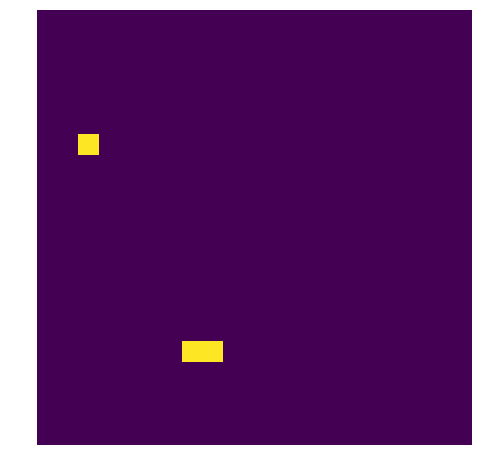
\includegraphics[width=3cm]{./Images/Chapter08/catch_v2} }}%
     \qquad
     \subfloat[\centering \texttt{Catch-v2}]{{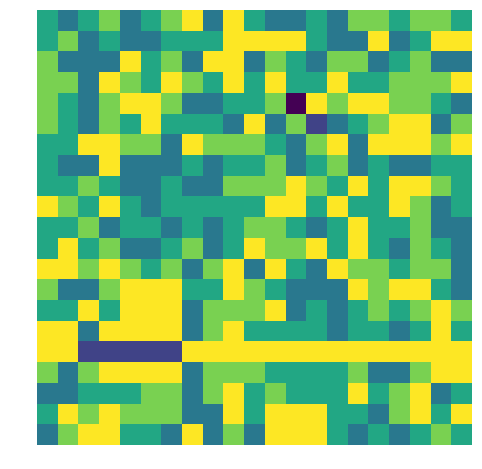
\includegraphics[width=3cm]{./Images/Chapter08/catch_v3} }}%
     \qquad
     \subfloat[\centering \texttt{Catch-v3}]{{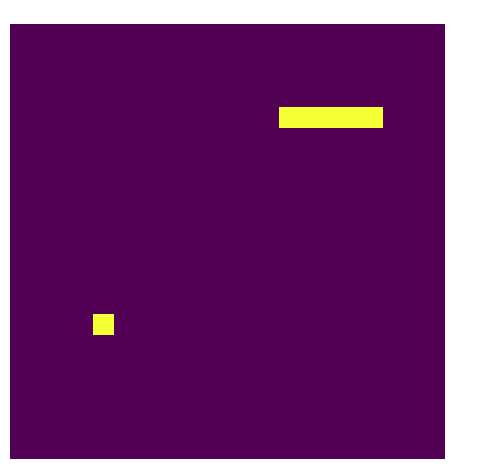
\includegraphics[width=3cm]{./Images/Chapter08/catch_v1} }}% 
    \caption{2 Figures side by side}
    \label{fig:catch_versions}%
\end{figure}

\paragraph{Experimental Setup}
Given the overall simplicity of the different \texttt{Catch} environments, we now train a DQN agent instead of the arguably more complex DQV and DDQN agents that we considered in Sec. \ref{}. The agent comes in the form a two-hidden layer convolutional neural network which is followed by a fully connected layer of $256$ hidden units preceding the final linear layer responsible for estimating the different $Q(s,a,)$ values. The first convolutional layer has $32$ channels whereas the second one has $64$ channels. All layers of the network are activated by a ReLU non-linearity. We use an experience replay memory buffer that is set to contain $400000$ trajectories, and start training the model as soon as $5000$ trajectories have been collected. For exploration purposes, we adopt the popular epsilon-greedy strategy with an initial $\epsilon$ value of $1$ which gets linearly annealed over time to $0.1$. Learning a near optimal policy on the aforementioned \texttt{Catch} environments with this type of DQN agent requires $\approx 5$ hours of training time. We visualize the learning curves for each of the four different \texttt{Catch} environments in Fig. \ref{}, where for every training iteration (reported on the $x$ axis) we report the average performance that is obtained by an agent that is evaluated on ten different episodes ($y$ axis). Shaded areas around the line plots correspond to $\pm 1$ std. deviation obtained over five different training runs with five different random seeds.    

\paragraph{DQN Performance}
As we can see from the results reported in Fig. \ref{}, the DQN agent described above is able to successfully learn a near optimal policy for all \texttt{Catch} versions. When it comes to \texttt{Catch-v0}, \texttt{Catch-v2} and \texttt{Catch-v3} we can observe that by the end of training the agent is able to catch $\approx 100\%$ of the falling balls, whereas its performance is slightly worse ($\approx 90\%$) when it comes to \texttt{Catch-v1} \footnote{Please note that the performance on \texttt{Catch-v1} can be improved by increasing the complexity of the DQN agent by adding one more convolutional layer. However, as the goal is to transfer the same type of model across \texttt{Catch} games we did not modify the architecture of the DQN agent, at the cost of having a slightly worse performing model.}. We can also observe that among the different \texttt{Catch} versions, \texttt{Catch-v0} and \texttt{Catch-v3} appear to be the easiest ones, as the agent requires significantly less training iterations to converge when compared to \texttt{Catch-v1} and \texttt{Catch-v2}. Furthermore, in line with the explanation presented beforehand, our results also confirm the hypothesis that \texttt{Catch-v2} is the overall most complicated \texttt{Catch} version, as learning requires significantly more, and potentially unstable, training iterations.

\begin{tikzpicture}
\begin{axis}
[	grid style={dashed,gray},
	grid = both, 
	tick style=black,
  	xlabel=Epochs,
	ylabel = $\%$ of caught balls,
	legend style={at={(-0.3,-0.3,-0.4)},anchor=south west,legend columns=4},
]

\addlegendentry{\texttt{Catch-v0}}

\addplot[blue, ultra thick] table[x=epochs,y=catchv0] {./Results/Chapter08/logs/catch_baselines.dat};
\addplot[name path=upper,draw=none, forget plot] table[x=epochs,y expr=\thisrow{catchv0}+\thisrow{stdv0}] {./Results/Chapter08/logs/catch_baselines.dat};
\addplot[name path=lower,draw=none, forget plot] table[x=epochs,y expr=\thisrow{catchv0}-\thisrow{stdv0}] {./Results/Chapter08/logs/catch_baselines.dat};
\addplot[fill=blue!10, forget plot] fill between[of=upper and lower];

\addlegendentry{\texttt{Catch-v1}}
\addplot[ultra thick, yellow] table[x=epochs,y=catchv3] {./Results/Chapter08/logs/catch_baselines.dat};
\addplot [name path=upper,draw=none, forget plot] table[x=epochs,y expr=\thisrow{catchv3}+\thisrow{stdv3}] {./Results/Chapter08/logs/catch_baselines.dat};
\addplot [name path=lower,draw=none, forget plot] table[x=epochs,y expr=\thisrow{catchv3}-\thisrow{stdv3}] {./Results/Chapter08/logs/catch_baselines.dat};
\addplot [fill=yellow!10, forget plot] fill between[of=upper and lower];

\addlegendentry{\texttt{Catch-v2}}
\addplot[ultra thick, red] table[x=epochs,y=catchv1] {./Results/Chapter08/logs/catch_baselines.dat};
\addplot[name path=upper,draw=none, forget plot] table[x=epochs,y expr=\thisrow{catchv1}+\thisrow{stdv1}] {./Results/Chapter08/logs/catch_baselines.dat};
\addplot[name path=lower,draw=none, forget plot] table[x=epochs,y expr=\thisrow{catchv1}-\thisrow{stdv1}] {./Results/Chapter08/logs/catch_baselines.dat};
\addplot[fill=red!10, forget plot] fill between[of=upper and lower];

\addlegendentry{\texttt{Catch-v3}}
\addplot[ultra thick, green] table[x=epochs,y=catchv2] {./Results/Chapter08/logs/catch_baselines.dat};
\addplot [name path=upper,draw=none, forget plot] table[x=epochs,y expr=\thisrow{catchv2}+\thisrow{stdv2}] {./Results/Chapter08/logs/catch_baselines.dat};
\addplot [name path=lower,draw=none, forget plot] table[x=epochs,y expr=\thisrow{catchv2}-\thisrow{stdv2}] {./Results/Chapter08/logs/catch_baselines.dat};
\addplot [fill=green!10, forget plot] fill between[of=upper and lower];

\end{axis}
\end{tikzpicture}



\subsection{From one Catch to Another}

 Replicate the study obtained when fine-tuning on Atari. Hypothesis that PT should be observed as 

\begin{figure}[ht!]
\resizebox{0.45\textwidth}{!}{  \centering
\begin{tikzpicture}
\begin{axis}
[	
	name=ax1,	
	grid style={dashed,gray},
	grid = both, 
	tick style=black,
  	xlabel=Epochs,
	ylabel = $\%$ of caught balls,
	title = \texttt{Catch-v0},
	legend pos=south east,	
]


%\addlegendentry{\texttt{Catch-v0}}
\addplot[blue, ultra thick] table[x=epochs,y=target_catch] {./Results/Chapter08/logs/catch_v0.dat};
\addplot [name path=upper,draw=none, forget plot] table[x=epochs,y expr=\thisrow{target_catch}+\thisrow{std_target_catch}] {./Results/Chapter08/logs/catch_v0.dat};
\addplot [name path=lower,draw=none, forget plot] table[x=epochs,y expr=\thisrow{target_catch}-\thisrow{std_target_catch}] {./Results/Chapter08/logs/catch_v0.dat};
\addplot [fill=blue!10, forget plot] fill between[of=upper and lower];

%\addlegendentry{\texttt{Catch-v1}}
\addplot[ultra thick, red] table[x=epochs,y=Catch_v2] {./Results/Chapter08/logs/catch_v0.dat};
\addplot [name path=upper,draw=none, forget plot] table[x=epochs,y expr=\thisrow{Catch_v2}+\thisrow{Catch_v2_std}] {./Results/Chapter08/logs/catch_v0.dat};
\addplot [name path=lower,draw=none, forget plot] table[x=epochs,y expr=\thisrow{Catch_v2}-\thisrow{Catch_v2_std}] {./Results/Chapter08/logs/catch_v0.dat};
\addplot [fill=red!10, forget plot] fill between[of=upper and lower];

%\addlegendentry{\texttt{Catch-v2}}
\addplot[ultra thick, green] table[x=epochs,y=Catch_v3] {./Results/Chapter08/logs/catch_v0.dat};
\addplot [name path=upper,draw=none, forget plot] table[x=epochs,y expr=\thisrow{Catch_v3}+\thisrow{Catch_v3_std}] {./Results/Chapter08/logs/catch_v0.dat};
\addplot [name path=lower,draw=none, forget plot] table[x=epochs,y expr=\thisrow{Catch_v3}-\thisrow{Catch_v3_std}] {./Results/Chapter08/logs/catch_v0.dat};
\addplot [fill=green!10, forget plot] fill between[of=upper and lower];

%\addlegendentry{\texttt{Catch-v3}}
\addplot[ultra thick, yellow] table[x=epochs,y=Catch_v4] {./Results/Chapter08/logs/catch_v0.dat};
\addplot [name path=upper,draw=none, forget plot] table[x=epochs,y expr=\thisrow{Catch_v4}+\thisrow{Catch_v4_std}] {./Results/Chapter08/logs/catch_v0.dat};
\addplot [name path=lower,draw=none, forget plot] table[x=epochs,y expr=\thisrow{Catch_v4}-\thisrow{Catch_v4_std}] {./Results/Chapter08/logs/catch_v0.dat};
\addplot [fill=yellow!10, forget plot] fill between[of=upper and lower];

\end{axis}


\begin{axis}
[	
	at={(ax1.south east)},
	xshift=1cm,
	grid style={dashed,gray},
	grid = both, 
	tick style=black,
  	xlabel=Epochs,
	%ylabel = $\%$ of caught balls,
	title = \texttt{Catch-v1},
	legend pos=south east,
]

%\addlegendentry{\texttt{Catch-v0}}

\addplot[yellow, ultra thick] table[x=epochs,y=target_catch] {./Results/Chapter08/logs/catch_v1.dat};
\addplot [name path=upper,draw=none, forget plot] table[x=epochs,y expr=\thisrow{target_catch}+\thisrow{std_target_catch}] {./Results/Chapter08/logs/catch_v1.dat};
\addplot [name path=lower,draw=none, forget plot] table[x=epochs,y expr=\thisrow{target_catch}-\thisrow{std_target_catch}] {./Results/Chapter08/logs/catch_v1.dat};
\addplot [fill=yellow!10, forget plot] fill between[of=upper and lower];

%\addlegendentry{\texttt{Catch-v2}}
\addplot[ultra thick, red] table[x=epochs,y=Catch_v0] {./Results/Chapter08/logs/catch_v1.dat};
\addplot [name path=upper,draw=none, forget plot] table[x=epochs,y expr=\thisrow{Catch_v0}+\thisrow{Catch_v0_std}] {./Results/Chapter08/logs/catch_v1.dat};
\addplot [name path=lower,draw=none, forget plot] table[x=epochs,y expr=\thisrow{Catch_v0}-\thisrow{Catch_v0_std}] {./Results/Chapter08/logs/catch_v1.dat};
\addplot [fill=red!10, forget plot] fill between[of=upper and lower];

%\addlegendentry{\texttt{Catch-v1}}
\addplot[ultra thick, green] table[x=epochs,y=Catch_v2] {./Results/Chapter08/logs/catch_v1.dat};
\addplot [name path=upper,draw=none, forget plot] table[x=epochs,y expr=\thisrow{Catch_v2}+\thisrow{Catch_v2_std}] {./Results/Chapter08/logs/catch_v1.dat};
\addplot [name path=lower,draw=none, forget plot] table[x=epochs,y expr=\thisrow{Catch_v2}-\thisrow{Catch_v2_std}] {./Results/Chapter08/logs/catch_v1.dat};
\addplot [fill=green!10, forget plot] fill between[of=upper and lower];

%\addlegendentry{\texttt{Catch-v3}}
\addplot[ultra thick, blue] table[x=epochs,y=Catch_v3] {./Results/Chapter08/logs/catch_v1.dat};
\addplot [name path=upper,draw=none, forget plot] table[x=epochs,y expr=\thisrow{Catch_v3}+\thisrow{Catch_v3_std}] {./Results/Chapter08/logs/catch_v1.dat};
\addplot [name path=lower,draw=none, forget plot] table[x=epochs,y expr=\thisrow{Catch_v3}-\thisrow{Catch_v3_std}] {./Results/Chapter08/logs/catch_v1.dat};
\addplot [fill=blue!10, forget plot] fill between[of=upper and lower];

\end{axis}


\begin{axis}
[	at={(ax1.south east)},
	xshift=9cm,
    grid style={dashed,gray},
	grid = both, 
	tick style=black,
  	xlabel=Epochs,
	%ylabel = $\%$ of caught balls,
	legend pos=south east,	
	title = \texttt{Catch-v2}
]


%\addlegendentry{\texttt{Catch-v0}}
\addplot[red, ultra thick] table[x=epochs,y=target_catch] {./Results/Chapter08/logs/catch_v2.dat};
\addplot [name path=upper,draw=none, forget plot] table[x=epochs,y expr=\thisrow{target_catch}+\thisrow{std_target_catch}] {./Results/Chapter08/logs/catch_v2.dat};
\addplot [name path=lower,draw=none, forget plot] table[x=epochs,y expr=\thisrow{target_catch}-\thisrow{std_target_catch}] {./Results/Chapter08/logs/catch_v2.dat};
\addplot [fill=red!10, forget plot] fill between[of=upper and lower];

%\addlegendentry{\texttt{Catch-v1}}
\addplot[ultra thick, blue] table[x=epochs,y=Catch_v0] {./Results/Chapter08/logs/catch_v2.dat};
\addplot [name path=upper,draw=none, forget plot] table[x=epochs,y expr=\thisrow{Catch_v0}+\thisrow{Catch_v0_std}] {./Results/Chapter08/logs/catch_v2.dat};
\addplot [name path=lower,draw=none, forget plot] table[x=epochs,y expr=\thisrow{Catch_v0}-\thisrow{Catch_v0_std}] {./Results/Chapter08/logs/catch_v2.dat};
\addplot [fill=blue!10, forget plot] fill between[of=upper and lower];

%\addlegendentry{\texttt{Catch-v2}}
\addplot[ultra thick, green] table[x=epochs,y=Catch_v3] {./Results/Chapter08/logs/catch_v2.dat};
\addplot [name path=upper,draw=none, forget plot] table[x=epochs,y expr=\thisrow{Catch_v3}+\thisrow{Catch_v3_std}] {./Results/Chapter08/logs/catch_v2.dat};
\addplot [name path=lower,draw=none, forget plot] table[x=epochs,y expr=\thisrow{Catch_v3}-\thisrow{Catch_v3_std}] {./Results/Chapter08/logs/catch_v2.dat};
\addplot [fill=green!10, forget plot] fill between[of=upper and lower];

%\addlegendentry{\texttt{Catch-v3}}
\addplot[ultra thick, yellow] table[x=epochs,y=Catch_v4] {./Results/Chapter08/logs/catch_v2.dat};
\addplot [name path=upper,draw=none, forget plot] table[x=epochs,y expr=\thisrow{Catch_v4}+\thisrow{Catch_v4_std}] {./Results/Chapter08/logs/catch_v2.dat};
\addplot [name path=lower,draw=none, forget plot] table[x=epochs,y expr=\thisrow{Catch_v4}-\thisrow{Catch_v4_std}] {./Results/Chapter08/logs/catch_v2.dat};
\addplot [fill=yellow!10, forget plot] fill between[of=upper and lower];

\end{axis}


\begin{axis}
[	
    at={(ax1.south east)},
	xshift=17cm,
    grid style={dashed,gray},
	grid = both, 
	tick style=black,
  	xlabel=Epochs,
	%ylabel = $\%$ of caught balls,
	%legend style={at={(-1,-0.4,-1.4)},anchor=south,legend columns=4},
	title= \texttt{Catch-v3}
]

\addlegendentry{\texttt{Catch-v0}}
\addplot[ultra thick, blue] table[x=epochs,y=Catch_v0] {./Results/Chapter08/logs/catch_v3.dat};
\addplot [name path=upper,draw=none, forget plot] table[x=epochs,y expr=\thisrow{Catch_v0}+\thisrow{Catch_v0_std}] {./Results/Chapter08/logs/catch_v3.dat};
\addplot [name path=lower,draw=none, forget plot] table[x=epochs,y expr=\thisrow{Catch_v0}-\thisrow{Catch_v0_std}] {./Results/Chapter08/logs/catch_v3.dat};
\addplot [fill=blue!10, forget plot] fill between[of=upper and lower];


\addlegendentry{\texttt{Catch-v1}}
\addplot[ultra thick, yellow] table[x=epochs,y=Catch_v4] {./Results/Chapter08/logs/catch_v3.dat};
\addplot [name path=upper,draw=none, forget plot] table[x=epochs,y expr=\thisrow{Catch_v4}+\thisrow{Catch_v4_std}] {./Results/Chapter08/logs/catch_v3.dat};
\addplot [name path=lower,draw=none, forget plot] table[x=epochs,y expr=\thisrow{Catch_v4}-\thisrow{Catch_v4_std}] {./Results/Chapter08/logs/catch_v3.dat};
\addplot [fill=yellow!10, forget plot] fill between[of=upper and lower];

\addlegendentry{\texttt{Catch-v2}}
\addplot[ultra thick, red] table[x=epochs,y=Catch_v2] {./Results/Chapter08/logs/catch_v3.dat};
\addplot [name path=upper,draw=none, forget plot] table[x=epochs,y expr=\thisrow{Catch_v2}+\thisrow{Catch_v2_std}] {./Results/Chapter08/logs/catch_v3.dat};
\addplot [name path=lower,draw=none, forget plot] table[x=epochs,y expr=\thisrow{Catch_v2}-\thisrow{Catch_v2_std}] {./Results/Chapter08/logs/catch_v3.dat};
\addplot [fill=red!10, forget plot] fill between[of=upper and lower];


\addlegendentry{\texttt{Catch-v3}}
\addplot[green, ultra thick] table[x=epochs,y=target_catch] {./Results/Chapter08/logs/catch_v3.dat};
\addplot [name path=upper,draw=none, forget plot] table[x=epochs,y expr=\thisrow{target_catch}+\thisrow{std_target_catch}] {./Results/Chapter08/logs/catch_v3.dat};
\addplot [name path=lower,draw=none, forget plot] table[x=epochs,y expr=\thisrow{target_catch}-\thisrow{std_target_catch}] {./Results/Chapter08/logs/catch_v3.dat};
\addplot [fill=green!10, forget plot] fill between[of=upper and lower];



\end{axis}


\end{tikzpicture}%
}
\caption{The results obtained after using a pre-trained \texttt{Catch} agent and fine-tuning it on a different \texttt{Catch} version. We can observe that despite all \texttt{Catch} versions being very similar no positive transfer is ever observed, as a model trained from scratch always outperforms a pre-trained, fine-tuned network.}
\label{fig:catch_transfer}
\end{figure}



\subsection{Self-Transfer}

 What happens if we perform self-transfer?
 When fine-tuned networks do not even self-transfer

\section{Deep-Q Networks Are Poor Feature Extractors}

 Explain the experiment designed with Pierre
 Results performance goes down and back up
 Conclusion has to be discussed with Pierre


